% latex table generated in R 2.15.3 by xtable 1.7-1 package
% Fri Sep  6 13:59:05 2013
\begin{table*}[ht]
\centering
\begin{tabular}{rp{15em}ccccc}
  \hline
Feature & Description & quant\_5 & mean & median & quant\_95 & histogram \\ 
  \hline
num\_commits & Number of commits in the pull request & 1.00 & 4.47 & 1.00 & 12.00 & 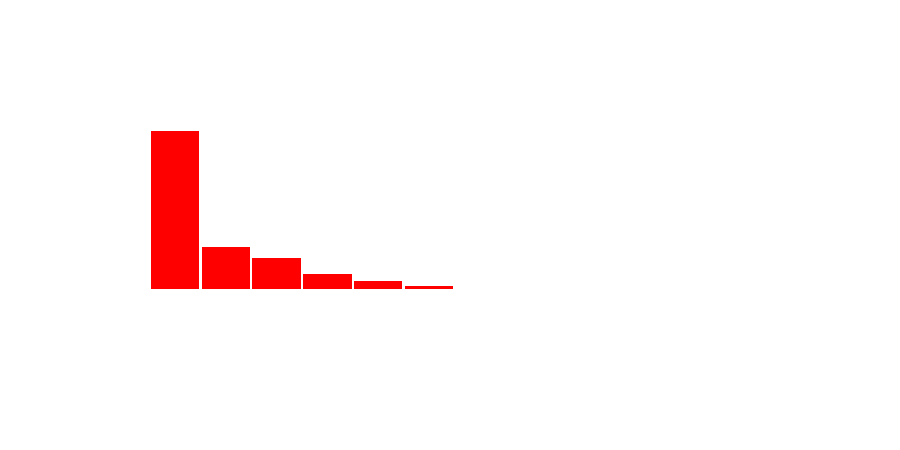
\includegraphics[scale = 0.1, clip = true, trim= 50px 60px 50px 60px]{hist-f128f3cb38588fe5202716588c047381.pdf} \\ 
  src\_churn & Number of lines changed (added + deleted) by the pull request. & 0.00 & 300.72 & 10.00 & 891.00 & 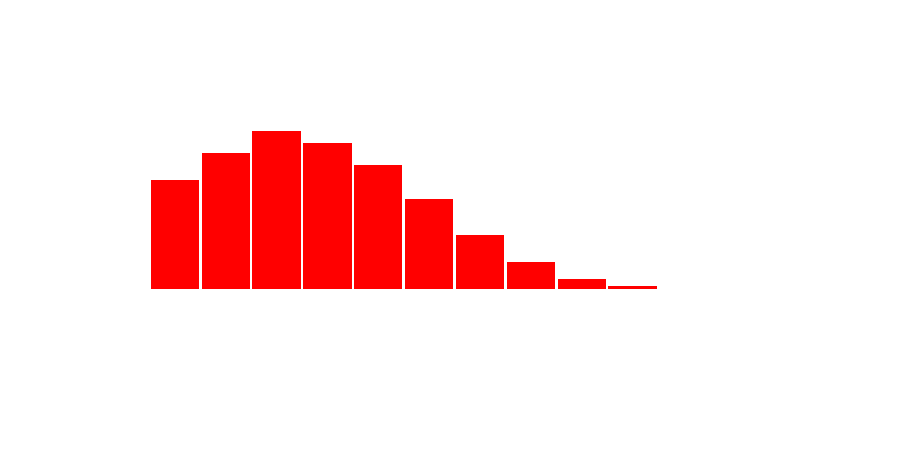
\includegraphics[scale = 0.1, clip = true, trim= 50px 60px 50px 60px]{hist-1f006c80a0da61518435a0c55f538326.pdf} \\ 
  test\_churn & Number of test lines changed in the pull request. & 0.00 & 88.88 & 0.00 & 282.00 & 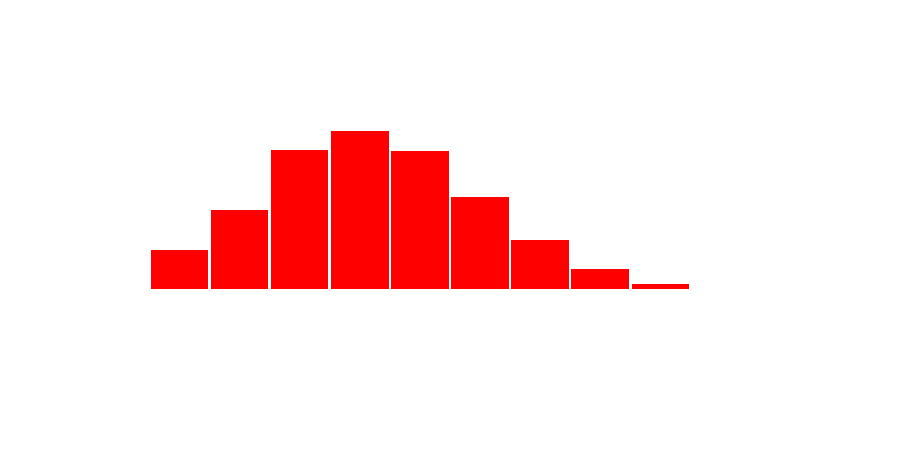
\includegraphics[scale = 0.1, clip = true, trim= 50px 60px 50px 60px]{hist-dd78ccaeedd7fc79735a66eb7f9e506b.pdf} \\ 
  files\_changed & Number of files touched by the pull request. & 1.00 & 12.12 & 2.00 & 31.00 & 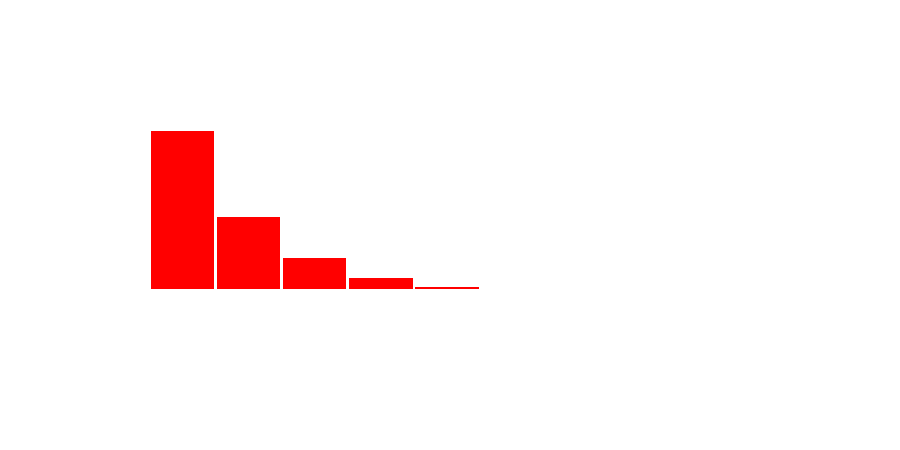
\includegraphics[scale = 0.1, clip = true, trim= 50px 60px 50px 60px]{hist-9b07b060359435635ff2bf4cd34f834a.pdf} \\ 
  num\_comments & The total number of comments (discussion and code review). & 0.00 & 2.77 & 1.00 & 12.00 & 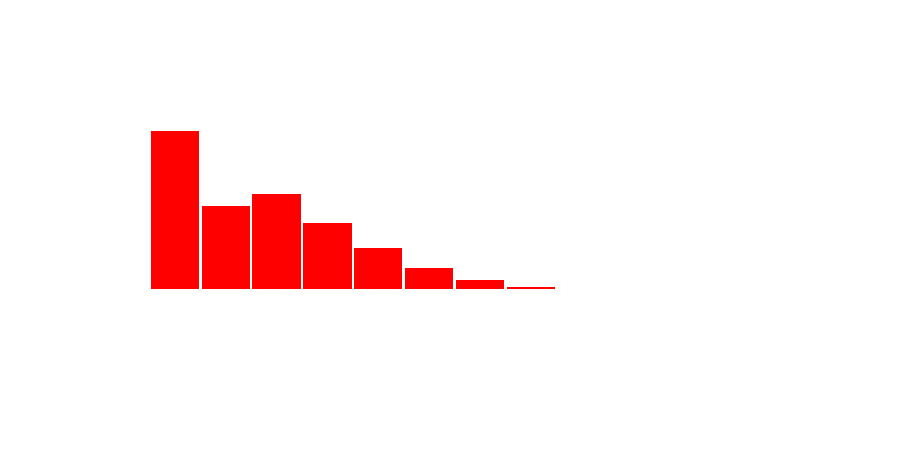
\includegraphics[scale = 0.1, clip = true, trim= 50px 60px 50px 60px]{hist-9db5e2b390de0d64d26c14798cb579ef.pdf} \\ 
  sloc & Executable lines of code at pull request merge time. & 1390.00 & 60897.87 & 26036.00 & 302156.00 & 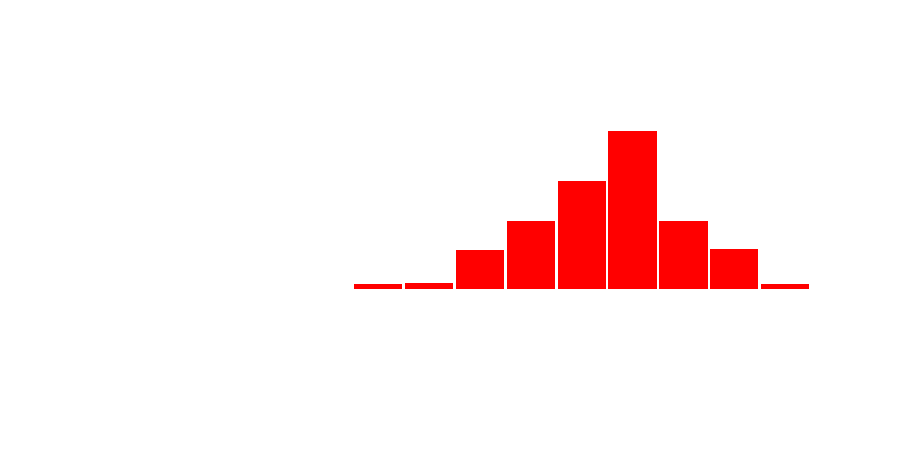
\includegraphics[scale = 0.1, clip = true, trim= 50px 60px 50px 60px]{hist-6b5159d3060b4fdf8493d4c818f79949.pdf} \\ 
  team\_size & Number of active core team members during the last 3 months prior the pull request creation. & 1.00 & 15.37 & 7.00 & 65.00 & 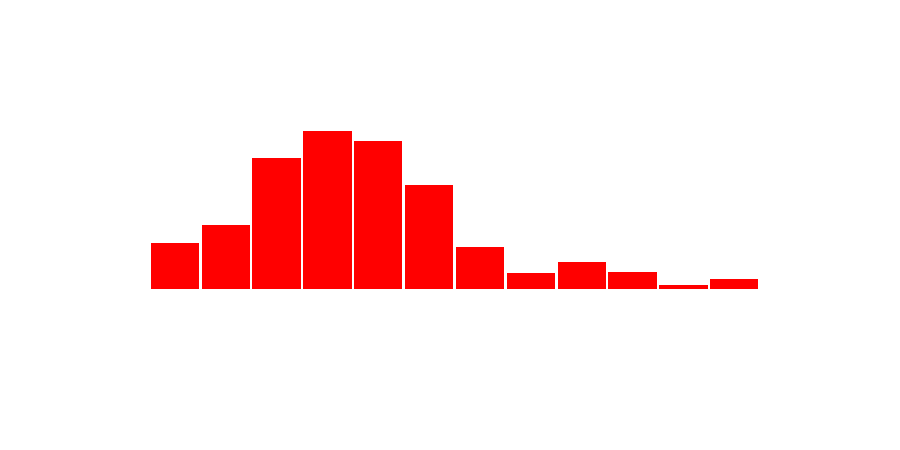
\includegraphics[scale = 0.1, clip = true, trim= 50px 60px 50px 60px]{hist-231fb4fabf4a3f0c551f2a97ae080508.pdf} \\ 
  perc\_external\_contribs & The ratio of commits from external members over core team members in the last 3 months prior to pull request creation. & 8.00 & 52.81 & 54.00 & 95.00 & 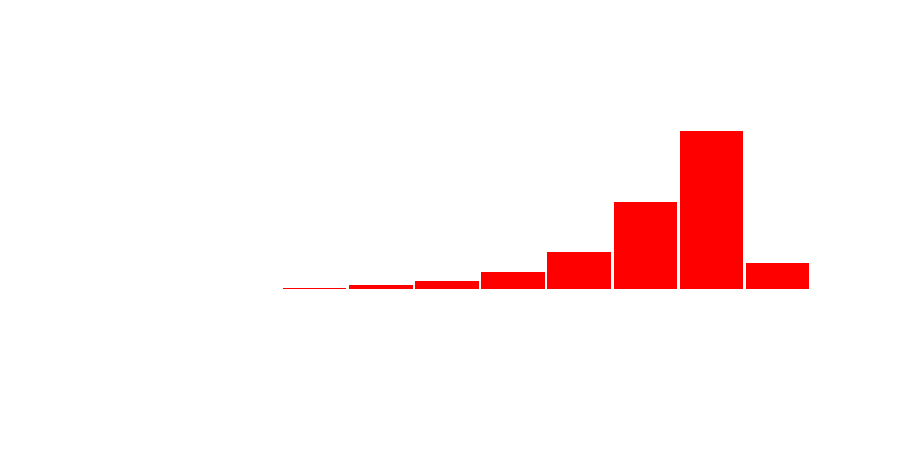
\includegraphics[scale = 0.1, clip = true, trim= 50px 60px 50px 60px]{hist-a222f0a5c377ba129dd6c8f257062591.pdf} \\ 
  commits\_on\_files\_touched & Number of total commits on files touched by the pull request 3 months before the pull request creation time. & 0.00 & 52.39 & 5.00 & 210.00 & 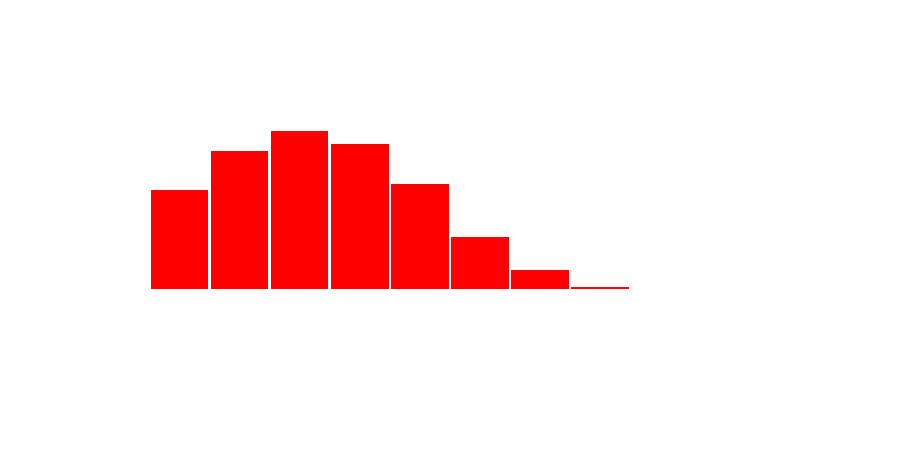
\includegraphics[scale = 0.1, clip = true, trim= 50px 60px 50px 60px]{hist-b735900ffcc37e7eda16dcd0c3497e6e.pdf} \\ 
  test\_lines\_per\_kloc & A proxy for the project's test coverage. & 1.39 & 1002.61 & 440.80 & 2147.43 & 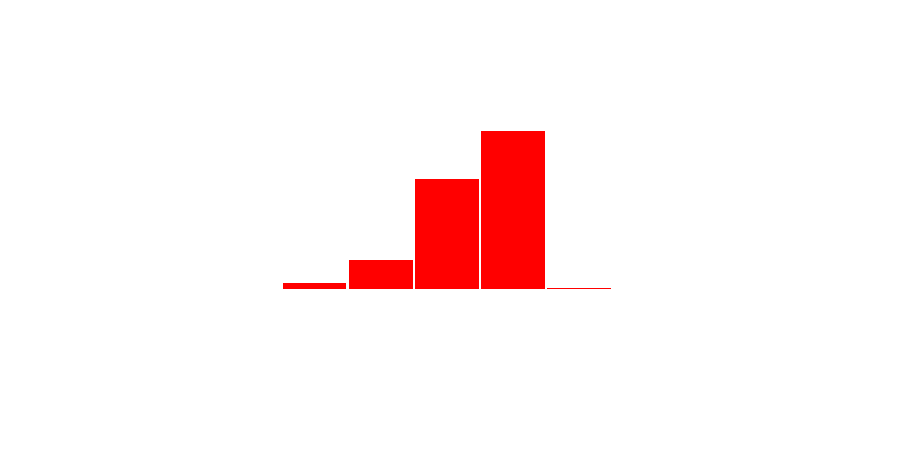
\includegraphics[scale = 0.1, clip = true, trim= 50px 60px 50px 60px]{hist-67ff3047089ba9ce0528884eab66e80a.pdf} \\ 
  prev\_pullreqs & Number of pull requests submitted by a specific developer, prior to the examined pull request. & 0.00 & 45.11 & 14.00 & 195.00 & 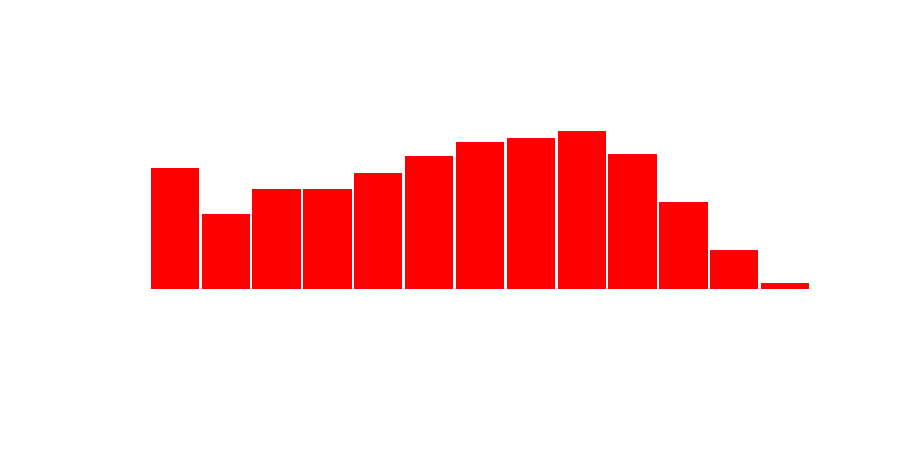
\includegraphics[scale = 0.1, clip = true, trim= 50px 60px 50px 60px]{hist-a2f7f60851dfa13cfbe0227d1d233767.pdf} \\ 
  requester\_succ\_rate & The percentage of the developer's pull requests that have been merged up to the creation of the examined pull request. & 0.00 & 0.59 & 0.78 & 1.00 & 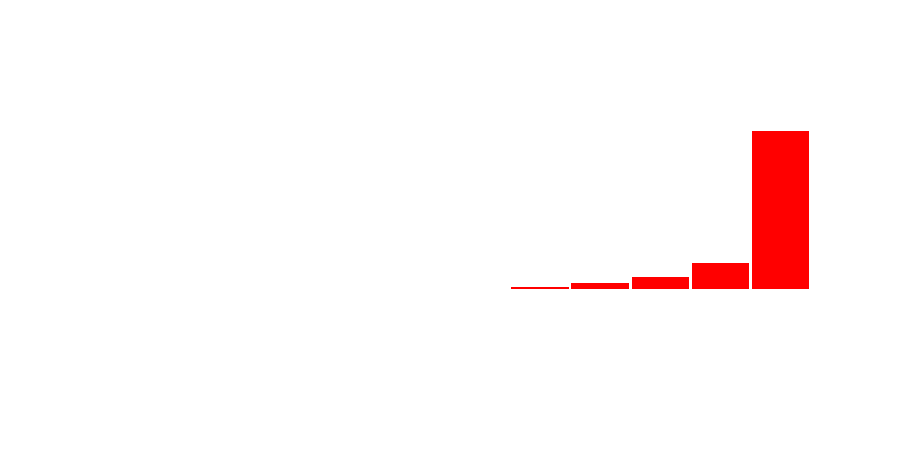
\includegraphics[scale = 0.1, clip = true, trim= 50px 60px 50px 60px]{hist-9363017165c3ded62457750f1c67c1af.pdf} \\ 
   \hline
\end{tabular}
\caption{Selected features and descriptive statistics. Historgrams are in log scale.} 
\label{tab:features}
\end{table*}
